\documentclass[border=3pt]{standalone}
\usepackage{amsmath,amssymb,tikz}
\usetikzlibrary{arrows.meta}
\pdfinfoomitdate=1
\pdftrailerid{}
\definecolor{ink}{HTML}{242E2C}
\definecolor{teal}{HTML}{386F79}
\definecolor{gold}{HTML}{A76C27}
\definecolor{slate}{HTML}{69798A}
\definecolor{berry}{HTML}{99606C}
\definecolor{quiet}{HTML}{9AA3A1}
\begin{document}

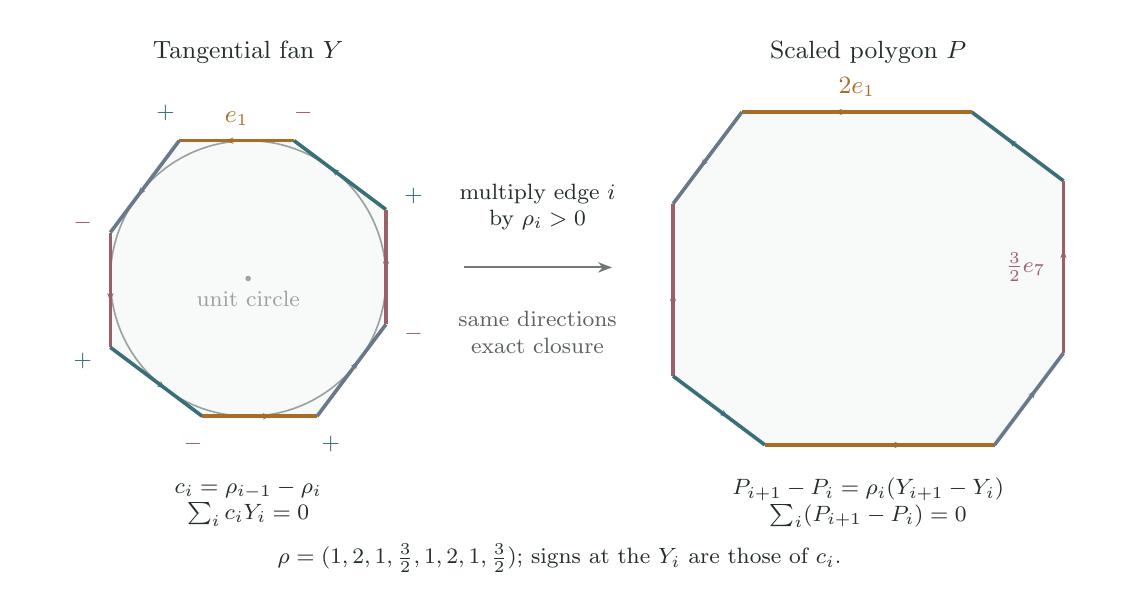
\begin{tikzpicture}[x=1.75cm,y=1.75cm,font=\small,text=ink]
\path[use as bounding box] (-1.60,-2.15) rectangle (6.15,1.82);
\coordinate (y0) at (1.000000000,0.500000000);
\coordinate (y1) at (0.333333333,1.000000000);
\coordinate (y2) at (-0.500000000,1.000000000);
\coordinate (y3) at (-1.000000000,0.333333333);
\coordinate (y4) at (-1.000000000,-0.500000000);
\coordinate (y5) at (-0.333333333,-1.000000000);
\coordinate (y6) at (0.500000000,-1.000000000);
\coordinate (y7) at (1.000000000,-0.333333333);
\coordinate (p0) at (5.916666667,0.708333333);
\coordinate (p1) at (5.250000000,1.208333333);
\coordinate (p2) at (3.583333333,1.208333333);
\coordinate (p3) at (3.083333333,0.541666667);
\coordinate (p4) at (3.083333333,-0.708333333);
\coordinate (p5) at (3.750000000,-1.208333333);
\coordinate (p6) at (5.416666667,-1.208333333);
\coordinate (p7) at (5.916666667,-0.541666667);
\fill[ink!3] (y0)--(y1)--(y2)--(y3)--(y4)--(y5)--(y6)--(y7)--cycle;
\fill[ink!3] (p0)--(p1)--(p2)--(p3)--(p4)--(p5)--(p6)--(p7)--cycle;
\draw[quiet,line width=.6pt] (0,0) circle[radius=1];
\fill[quiet] (0,0) circle[radius=1pt];
\node[text=quiet,font=\footnotesize] at (0,-.15) {unit circle};
\draw[teal,line width=1.3pt] (y0)--(y1);
\draw[teal,line width=1.3pt] (p0)--(p1);
\draw[teal,-{Stealth[length=3pt]},line width=.65pt] (0.733333333,0.700000000)--(0.600000000,0.800000000);
\draw[teal,-{Stealth[length=3pt]},line width=.65pt] (5.650000000,0.908333333)--(5.516666667,1.008333333);
\node[font=\footnotesize,text=teal] at (1.200000000,0.600000000) {$+$};
\draw[gold,line width=1.3pt] (y1)--(y2);
\draw[gold,line width=1.3pt] (p1)--(p2);
\draw[gold,-{Stealth[length=3pt]},line width=.65pt] (0.000000000,1.000000000)--(-0.166666667,1.000000000);
\draw[gold,-{Stealth[length=3pt]},line width=.65pt] (4.583333333,1.208333333)--(4.250000000,1.208333333);
\node[font=\footnotesize,text=berry] at (0.400000000,1.200000000) {$-$};
\draw[slate,line width=1.3pt] (y2)--(y3);
\draw[slate,line width=1.3pt] (p2)--(p3);
\draw[slate,-{Stealth[length=3pt]},line width=.65pt] (-0.700000000,0.733333333)--(-0.800000000,0.600000000);
\draw[slate,-{Stealth[length=3pt]},line width=.65pt] (3.383333333,0.941666667)--(3.283333333,0.808333333);
\node[font=\footnotesize,text=teal] at (-0.600000000,1.200000000) {$+$};
\draw[berry,line width=1.3pt] (y3)--(y4);
\draw[berry,line width=1.3pt] (p3)--(p4);
\draw[berry,-{Stealth[length=3pt]},line width=.65pt] (-1.000000000,0.000000000)--(-1.000000000,-0.166666667);
\draw[berry,-{Stealth[length=3pt]},line width=.65pt] (3.083333333,0.041666667)--(3.083333333,-0.208333333);
\node[font=\footnotesize,text=berry] at (-1.200000000,0.400000000) {$-$};
\draw[teal,line width=1.3pt] (y4)--(y5);
\draw[teal,line width=1.3pt] (p4)--(p5);
\draw[teal,-{Stealth[length=3pt]},line width=.65pt] (-0.733333333,-0.700000000)--(-0.600000000,-0.800000000);
\draw[teal,-{Stealth[length=3pt]},line width=.65pt] (3.350000000,-0.908333333)--(3.483333333,-1.008333333);
\node[font=\footnotesize,text=teal] at (-1.200000000,-0.600000000) {$+$};
\draw[gold,line width=1.3pt] (y5)--(y6);
\draw[gold,line width=1.3pt] (p5)--(p6);
\draw[gold,-{Stealth[length=3pt]},line width=.65pt] (0.000000000,-1.000000000)--(0.166666667,-1.000000000);
\draw[gold,-{Stealth[length=3pt]},line width=.65pt] (4.416666667,-1.208333333)--(4.750000000,-1.208333333);
\node[font=\footnotesize,text=berry] at (-0.400000000,-1.200000000) {$-$};
\draw[slate,line width=1.3pt] (y6)--(y7);
\draw[slate,line width=1.3pt] (p6)--(p7);
\draw[slate,-{Stealth[length=3pt]},line width=.65pt] (0.700000000,-0.733333333)--(0.800000000,-0.600000000);
\draw[slate,-{Stealth[length=3pt]},line width=.65pt] (5.616666667,-0.941666667)--(5.716666667,-0.808333333);
\node[font=\footnotesize,text=teal] at (0.600000000,-1.200000000) {$+$};
\draw[berry,line width=1.3pt] (y7)--(y0);
\draw[berry,line width=1.3pt] (p7)--(p0);
\draw[berry,-{Stealth[length=3pt]},line width=.65pt] (1.000000000,0.000000000)--(1.000000000,0.166666667);
\draw[berry,-{Stealth[length=3pt]},line width=.65pt] (5.916666667,-0.041666667)--(5.916666667,0.208333333);
\node[font=\footnotesize,text=berry] at (1.200000000,-0.400000000) {$-$};
\node at (0,1.64) {Tangential fan $Y$};
\node at (4.5,1.64) {Scaled polygon $P$};
\draw[ink!65,-{Stealth[length=5pt]},line width=.7pt] (1.57,.08)--(2.64,.08);
\node[align=center,font=\footnotesize] at (2.10,.52) {multiply edge $i$\\by $\rho_i>0$};
\node[align=center,font=\footnotesize,text=ink!75] at (2.10,-.39) {same directions\\exact closure};
\node[above=2pt,text=gold] at (-.083333,1) {$e_1$};
\node[above=2pt,text=gold] at (4.416667,1.208333) {$2e_1$};
\node[text=berry,left=3pt,font=\footnotesize] at (5.916667,.083333) {$\tfrac32 e_7$};
\node[align=center,font=\footnotesize] at (0,-1.63) {$c_i=\rho_{i-1}-\rho_i$\\$\sum_i c_iY_i=0$};
\node[align=center,font=\footnotesize] at (4.5,-1.63)
  {$P_{i+1}-P_i=\rho_i(Y_{i+1}-Y_i)$\\$\sum_i(P_{i+1}-P_i)=0$};
\node[font=\footnotesize] at (2.26,-2.03)
  {$\rho=(1,2,1,\tfrac32,1,2,1,\tfrac32)$; signs at the $Y_i$ are those of $c_i$.};
\end{tikzpicture}
\end{document}
